%% Application à des données réelles
% le Sweaveopt


\chapter{Application à des données réelles}
\label{chap:application} 

Pour mettre en application l'approche proposée par \textit{chavez2016extreme***}, deux jeux de données du paquetage \texttt{CASdatasets} sont utilisés. Soit \texttt{auscathist} et \texttt{nzcathist}. Ces données représentent respectivement l'historique des catastrophes naturelles pour l'Australie ainsi que pour la Nouvelle-Zélande. Les deux jeux de données contiennent également différentes statistiques de ces catastrophes. Voici une liste des variables disponibles:
\begin{itemize}
\item \texttt{Year}: l'année d'occurence de la catastrophe.
\item \texttt{Quarter}: le trimestre d'occurence de la catastrophne.
\item \texttt{Date}: la date d'occurence complète de la catastrophe.
\item \texttt{FirstDay}: la date de la première journée d'occurence de la catastrophe.
\item \texttt{LastDay}: la date de la dernière journée de la catastrophe (seulement disponible pour l'Australie).
\item \texttt{Event}: une description de la catastrophe.
\item \texttt{Type}: le type de catastrophe.
\item \texttt{Location}: une description du lieu de la catastrophe.
\item \texttt{OriginalCost}: coût original de la catastrophe en millions de \textit{AUD} ou \textit{NZD}.
\item \texttt{NormCost2011}: coût normalisé en millions de dollars de 2011 (inflation, richesse et population).
\item \texttt{NormCost2014}: coût normalisé en millions de dollars de 2014 (inflation, richesse et population).
\end{itemize}
\

Les tables \ref{tab:3.1} et \ref{tab:3.2} contiennent un résumé statistique des données australiennes:

% latex table generated in R 3.6.1 by xtable 1.8-4 package
% Thu Nov 14 22:18:50 2019
\begin{table}[ht]
\centering
\begin{tabular}{cccccccc}
  \hline
 & Mean & Std.Dev & Min & Median & Max & N.Valid & Pct.Valid \\ 
  \hline
NormCost2011 & 254 & 589 & 2 & 66 & 4296 & 190 & 92 \\ 
  NormCost2014 & 288 & 639 & 2 & 77 & 4606 & 206 & 100 \\ 
  OriginalCost & 104 & 295 & 1 & 15 & 2388 & 206 & 100 \\ 
  Quarter & 2 & 1 & 1 & 2 & 4 & 206 & 100 \\ 
  Year & 1995 & 12 & 1967 & 1998 & 2014 & 206 & 100 \\ 
   \hline
\end{tabular}
\caption{Résumé statistique des variables numériques pour l'Australie} 
\label{tab:3.1}
\end{table}% latex table generated in R 3.6.1 by xtable 1.8-4 package
% Thu Nov 14 22:18:50 2019
\begin{table}[ht]
\centering
\begin{tabular}{cccccc}
  \hline
 & Freq & \% Valid & \% Valid Cum. & \% Total & \% Total Cum. \\ 
  \hline
Bushfire & 26 & 13 & 13 & 13 & 13 \\ 
  Cyclone & 33 & 16 & 29 & 16 & 29 \\ 
  Earthquake & 4 & 2 & 31 & 2 & 31 \\ 
  Flood & 25 & 12 & 43 & 12 & 43 \\ 
  Flood, Storm & 27 & 13 & 56 & 13 & 56 \\ 
  Hailstorm & 33 & 16 & 72 & 16 & 72 \\ 
  Other & 3 & 1 & 73 & 1 & 73 \\ 
  Storm & 54 & 26 & 100 & 26 & 100 \\ 
  Tornado & 1 & 0 & 100 & 0 & 100 \\ 
  $<$NA$>$ & 0 &  &  & 0 & 100 \\ 
  Total & 206 & 100 & 100 & 100 & 100 \\ 
   \hline
\end{tabular}
\caption{Distribution du Type de catastrophe pour l'Australie} 
\label{tab:3.2}
\end{table}
Les tables \ref{tab:3.3} et \ref{tab:3.4} contiennent le même type de résumé pour la Nouvelle-Zélande:
% latex table generated in R 3.6.1 by xtable 1.8-4 package
% Thu Nov 14 22:18:50 2019
\begin{table}[ht]
\centering
\begin{tabular}{cccccccc}
  \hline
 & Mean & Std.Dev & Min & Median & Max & N.Valid & Pct.Valid \\ 
  \hline
NormCost2011 & 17 & 41 & 0 & 5 & 371 & 129 & 89 \\ 
  NormCost2014 & 138 & 1437 & 0 & 6 & 17321 & 145 & 100 \\ 
  OriginalCost & 125 & 1370 & 0 & 4 & 16500 & 145 & 100 \\ 
  Quarter & 2 & 1 & 1 & 2 & 4 & 145 & 100 \\ 
  Year & 1999 & 11 & 1968 & 2001 & 2014 & 145 & 100 \\ 
   \hline
\end{tabular}
\caption{Résumé statistique des variables numériques pour la Nouvelle-Zélande} 
\label{tab:3.3}
\end{table}% latex table generated in R 3.6.1 by xtable 1.8-4 package
% Thu Nov 14 22:18:50 2019
\begin{table}[ht]
\centering
\begin{tabular}{cccccc}
  \hline
 & Freq & \% Valid & \% Valid Cum. & \% Total & \% Total Cum. \\ 
  \hline
Cyclone & 4 & 3 & 3 & 3 & 3 \\ 
  Earthquake & 7 & 5 & 8 & 5 & 8 \\ 
  Flood & 58 & 40 & 48 & 40 & 48 \\ 
  Flood, Storm & 9 & 6 & 54 & 6 & 54 \\ 
  Hailstorm & 8 & 6 & 59 & 6 & 59 \\ 
  Other & 10 & 7 & 66 & 7 & 66 \\ 
  Power outage & 2 & 1 & 68 & 1 & 68 \\ 
  Storm & 32 & 22 & 90 & 22 & 90 \\ 
  Tornado & 11 & 8 & 97 & 8 & 97 \\ 
  Weather & 4 & 3 & 100 & 3 & 100 \\ 
  $<$NA$>$ & 0 &  &  & 0 & 100 \\ 
  Total & 145 & 100 & 100 & 100 & 100 \\ 
   \hline
\end{tabular}
\caption{Distribution du Type de catastrophe pour la Nouvelle-Zélande} 
\label{tab:3.4}
\end{table}\

Pour chaque jeu de données, une nouvelle variable du montant de catastrophe est créée à partir de la variable \texttt{NormCost2014} (\texttt{CostUS2019}). Cette nouvelle variable représente le coût ajusté au niveau du 30 juin 2019 en considérant l'indice du prix à la consommation de chaque pays et le coût est également converti en dollar américain. La table \ref{tab:3.5} contient les chiffres utilisés \footnote{https://www.rateinflation.com/consumer-price-index  \newline https://www.exchange-rates.org/Rate/AUD/USD/6-30-2019}.

% latex table generated in R 3.6.1 by xtable 1.8-4 package
% Thu Nov 14 22:18:50 2019
\begin{table}[ht]
\centering
\begin{tabular}{cccc}
  \hline
 & IPC 2014 & IPC 2019 & Taux de change 2019 \\ 
  \hline
AUS & 105.9000 & 114.8000 & 0.7031 \\ 
  NZ & 974.7000 & 1039.0000 & 0.6722 \\ 
   \hline
\end{tabular}
\caption{Valeurs utilisées pour CostUS2019} 
\label{tab:3.5}
\end{table}\

Étant donné que les deux jeux de données sont très semblables, ceux-ci sont regroupés en un seul jeu de données et une variable \texttt{Country} est rajoutée. Étant donné le nombre limité de données disponibles et pour rendre l'analyse pertinente et possible, seulement les variables \texttt{CostUS2019}, \texttt{Year}, \texttt{Country} et \texttt{Type} sont conservées. Les figures \ref{fig:3.1}, \ref{fig:3.2}, \ref{fig:3.3} et \ref{fig:3.4} résument bien le jeu de données final utilisé pour l'analyse.


\begin{figure}
\begin{center}
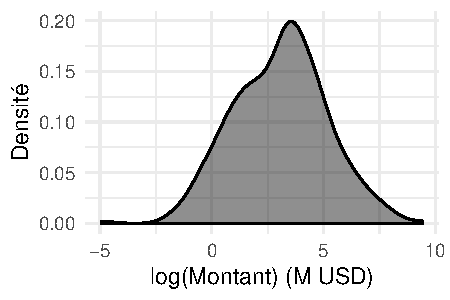
\includegraphics{images/fig-plot1}
\end{center}
\caption{Densité du logarithme du montant des catastrophes}
\label{fig:3.1}
\end{figure}


